\section{Theory}
The Four-Probe method is a widely used technique in materials science and condensed matter physics for accurate measurement of resistivity in materials. It is preferred over the conventional Two-Probe method due to its inherent advantages in minimizing errors caused by contact resistance. Four equally spaced collinear probes are used to make electrical contact with the surface of the material, with separate pairs of terminals to carry current and sense voltage. This configuration allows for precise voltage and current measurements, independent of the contact resistance, leading to more accurate and reliable resistivity measurements.

To set up a Four-Probe measurement, the probes are carefully positioned on the sample surface, to form a known probe spacing. A known current is passed through the outer probes, and the voltage drop across the inner probes is measured as shown in Fig. \ref{t1}. The resistivity of the material can then be calculated using the measured voltage and current values, along with the probe spacing and geometry, following established mathematical formulas, such as the Van der Pauw method.
		
The Four-Probe method offers several advantages over the Two-Probe method. Firstly, it eliminates errors associated with contact resistance, which can be a significant source of inaccuracy in resistivity measurements. Secondly, it allows for precise and simultaneous voltage and current measurements, leading to improved accuracy and reproducibility. Additionally, the Four-Probe method can be used to measure resistivity in a wide range of materials, including thin films, bulk samples, and even highly resistive materials. Overall, the Four-Probe method is a reliable and widely used technique for accurate resistivity measurements in materials research and characterization.
		
\begin{figure}
    \centering
    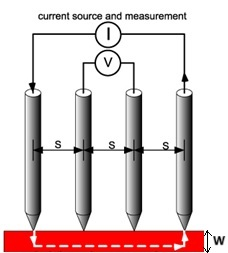
\includegraphics[width=0.5\columnwidth]{images/t1.jpg}
    \caption{Schematic of the Four-Probe setup}
    \label{t1}
\end{figure}

\subsection{Mathematical Formulation}
\subsubsection*{For semi-infinite conducting material}
A hemispherical equipotential surface develops at a probe when current flowing from a semi-infinite material is dispersed isotropically. The potential drop at an inner probe when two probes of different distances and opposing polarity are considered is:

\begin{align}
    V = \frac{\rho_0I}{2\pi}\left(\frac{1}{r_1}-\frac{1}{r_2}\right)
\end{align}

where $\rho_0$ is the resistivity, $I$ is the current passed through the outer electrode and $r_1$ and $r_2$ is the distance from the probe $1$ and probe $4$ respectively. The floating potential across the inner terminals is determined by the following equation when evenly spaced probes are taken into account.

\begin{align}V=\frac{\rho_0I}{2\pi S}\end{align}

S is the probe spacing. The resistivity of the material can be calculated using the following equation:

\begin{align} \label{e1}
    \rho_0 = \frac{V}{I} 2\pi S
\end{align}

\begin{figure*}
    \centering
    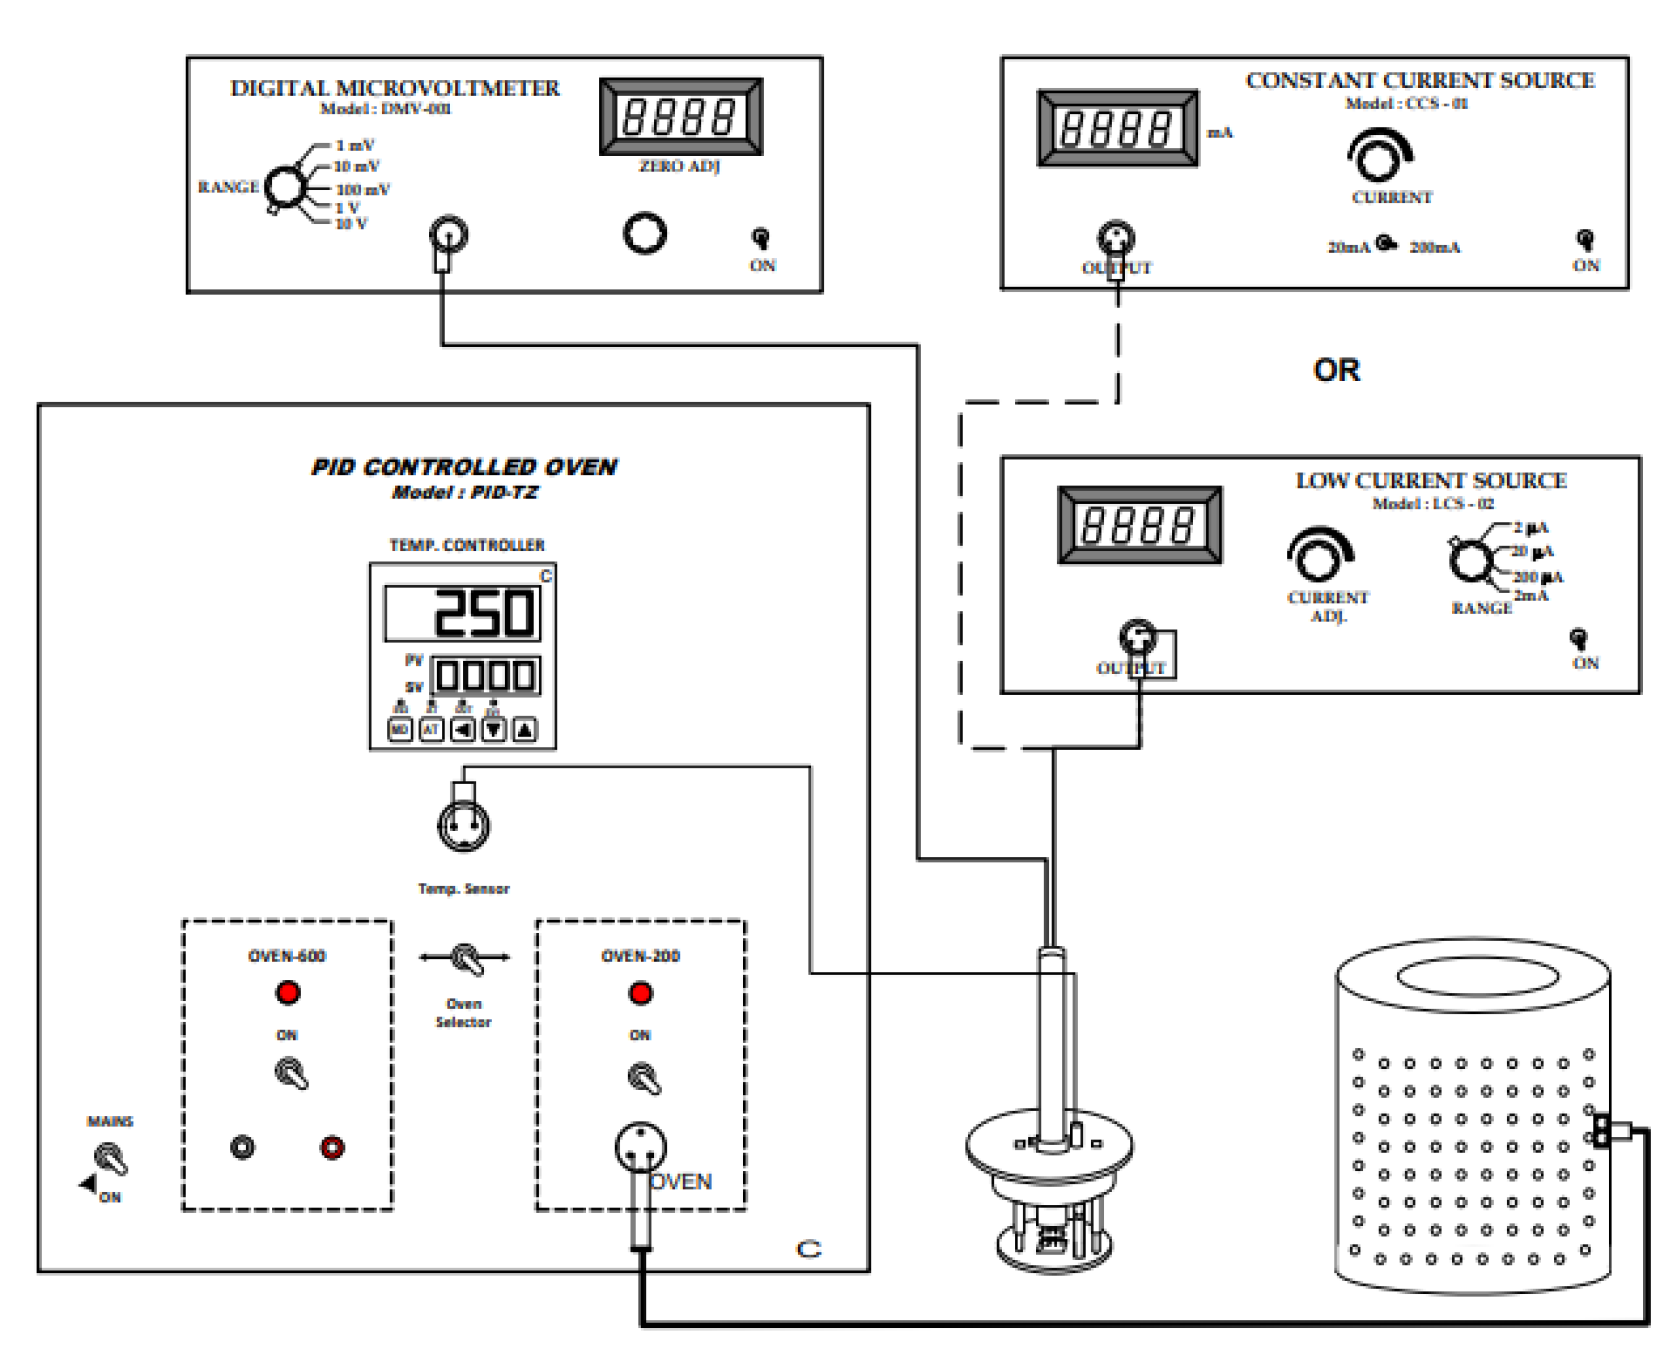
\includegraphics[width=1.3\columnwidth]{images/expt.png}
    \caption{Experimental setup for resistivity measurement with Four-Probe method}
\end{figure*}

\subsubsection*{For thin sheet placed on a non-conducting surface}
Since the thickness of the samples are small compared to the probe distance, a correction factor for it has to be applied. If the bottom surface is not conducting, then the corrected formula for resistivity will be:

\begin{align}\rho = \frac{\rho_0}{G_7(\sfrac{W}{S})}\end{align}

where $W$ is the width of the sample and $G_7(\sfrac{W}{S})$ is the required correction factor dependent
on the width-to-spacing ratio $\sfrac{W}{S}$, defined as follows:

\begin{align}
    G_7(\sfrac{W}{S}) = 1 + 4 \frac{S}{W}\sum_{n=1}^{\infty} f(S,\;W,\;n) 
\end{align}

\begin{align}
    f(S,\;W,\;n) = \left[\frac{1}{\sqrt{\left(\frac{S}{W}\right)^2+n^2}} - \frac{1}{\sqrt{\left(\frac{2S}{W}\right)^2+4n^2}}\right]
\end{align}

For smaller values of $W/S (\le 0.25)$, we can approximate the value of $G_7(\sfrac{W}{S})$ as:

\begin{align}
    G_7(\sfrac{W}{S}) = \frac{2S}{W}\ln(2)
\end{align}

Thus, for samples where $W/S \le 0.25$ or for sample thicknesses up to 0.5 mm, the correction factor can be directly obtained from the above equation.
For the given experiment, considering $S = 2$ mm
and $W = 0.5$ mm for Ge and Si and $\sim 0.017$ mm for Al, the correction factor is can be obtained from the above equation. Thus we get,

\begin{equation}\label{e2}
    \rho = \frac{\pi}{\ln(2)}W\frac{V}{I}
\end{equation}

\subsection{Temperature dependence of Resistivity}
The temperature dependence of resistivity varies for all three different types of materials we use.
\begin{figure}[H]
    \centering
    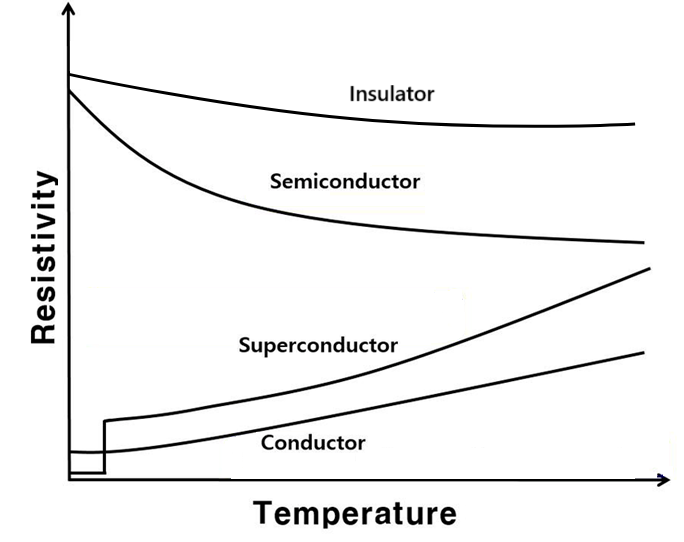
\includegraphics[width=.8\columnwidth]{images/t2.png}
    \caption{A simplied plot depicting the relationship between temperature and resistivity for three types of materials}
\end{figure}

The resistance of the conductor increase with the increase in temperature because of the increased collision between electrons \& vibrating lattice ions (phonons), which impede their flow and lead to resistance. The temperature coefficient of resistance of the metallic substance is positive.

In semiconductors, the numbers of free electrons in the valence band increase because of the breaking of the covalent bond at increased temperature. 

Thus, more electrons from the valence band reach the conduction band. As a result, the resistance of the semiconductor material decrease with an increase in temperature. 
Similarly, the resistance of the insulating material decrease with an increase in temperature (but quite slowly w.r.t. semi-conductors). Fig. 3 roughly shows the relationship between the change in the resistance and temperature rise for the three categories of material.

\subsubsection*{Relation of resistivity the band gap of a
semiconductor}

If $E_g$ is the band gap energy, $k_B = 8.6\times 10^{-5}$ eV/K is the Boltzmann constant, and $T$ is the temperature in Kelvin,

\begin{equation}\label{e3}
    E_g = 2k_B\frac{\ln(\rho)}{\sfrac{1}{T}}
\end{equation}

where $\frac{\ln(\rho)}{\sfrac{1}{T}}$ can be determined from the slope of as appropriate $\ln(\rho)$ vs. $T^{-1}$ plot.
% =====================================================
\section{Experimental Setup}

\subsection*{Apparatus}

\begin{enumerate}
    \item Four-Probe arrangement with spring-loaded probes
    \item PID-controlled oven for temperature regulation
    \item Constant current source (for both low and high current ranges)
    \item Digital microvoltmeter
    \item Thermocouple for temperature sensing
    \item Aluminum and semiconductor samples (n-Si, n-Ge)
    \item Screw Gauge\\
\end{enumerate}

\begin{figure}
    \centering
    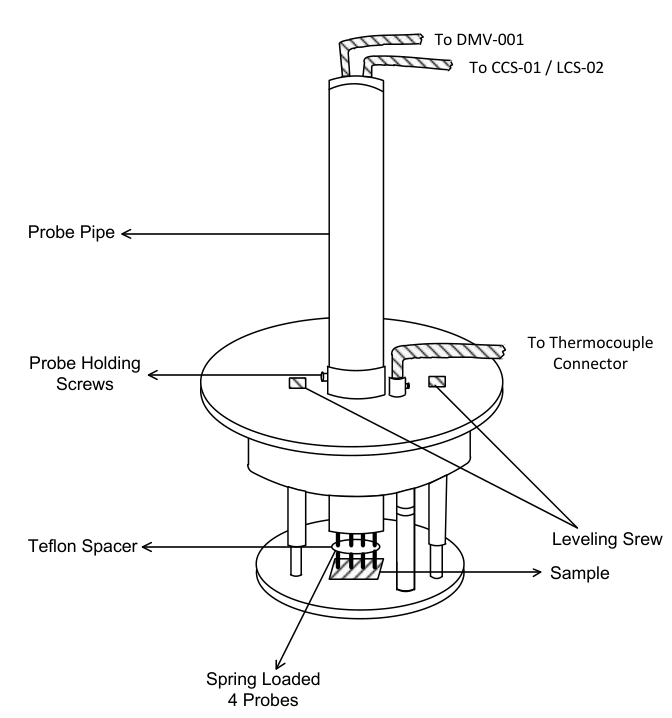
\includegraphics[width=1\columnwidth]{images/setup.png}
    \caption{The Four-Probe setup}
\end{figure}

The connections were made as shown in Fig. 2 and 4. The sample was placed on a non-conducting surface, and the four probes were gently rested on the sample and tightened in position. The voltage (V) and current (I) measurements were taken from the respective digital displays.

When temperature changes were required, the sample setup was lowered into the oven chamber, and the thermocouple sensor and oven socket were connected to the PID (Proportional-Integral-Derivative) controller. After selecting the desired oven temperature (e.g., 200°C) and turning on the mains, data collection was initiated once the Present Value (PV) stabilized to the Set Value (SV) on the PID controller.